\chapter{Analýza pomocí metody 4ftMiner}
\label{ch:cleverminer}

Pomocí metody 4ftMiner, která je jednou z metod procedury GUHA jsem provedla analýzu shrinků produktu. Tato metoda je implemnetovaná v  knihovně \emph{Cleverminer} pro jazyk Python. Pracovala jsem pouze se vzorem dat jednoho měsíce a s kategorií produktů \emph{Velmi čerstvé}, zastoupena 48, \% a \emph{Čerstvé}, zastoupena 52 \%. Princip metod, které se používají v knihovně, a důležité pojmy týkající se GUHA procedur jsou popsány v sekci \ref*{sec:Teorie:Guha}. 

Zkoumaný dataset se záznamy shrinků produktů jsem rozšířila o další sledované sloupce, které dávají do srovnání hodnotu shrinku a objem tržeb. Vytvořila jsem takto sloupce: podíl shrinku na celkových tržbách prodejny, podíl shrinku na tržbách shrinkovaného produktu na prodejně, podíl shrinku a tržeb v kategorii úrovně 1.

Na základě zastoupení jednotlivých typů shrinků, kde prošlé a zkažené zboží zaujímá téměř 65 \% shrinků, se následující analýzy zaměřují pouze na tento typ, viz tab. \ref*{tab:shrinkyZastoupeni}.

\begin{table}[hbtp!]
    \begin{center}
            \captionsetup{justification=centering}
    \caption{Zastoupení vybraných shrinků ve zkoumaných datech \\(kategorie Čertvé a Velmi čerstvé).}
    \begin{tabular}{l r}
        Typ shrinku & Zastoupení v kategoriích [\%]\\
        \midrule
        Prošlé a zkažené zboží & $64{,}97$ \\
        Potravinová banka & $23{,}72$ \\
         Poškození & $6{,}26$ \\
        Zvířecí útulky & $2{,}69$ \\
        Kompostéry &  $2{,}36$ \\
        \end{tabular}
    \label{tab:shrinkyZastoupeni}
\end{center}
\end{table}

Metoda pracuje pouze s kategorickými hodnotami, proto bylo nutné kategorizovat sloupce s hodnotou shrinku, s množstvím shrinkovaných produktů a s jednotlivými podíly. Na obrázcích \ref*{obr:nb:hist} až \ref{obr:nb:hist5} jsou zobrazené četnosti záznamů v kategoriích.

\begin{figure}[h!]
    \centering
    \begin{minipage}[b]{.55\textwidth}
      \centering
      \captionsetup{justification=centering}

      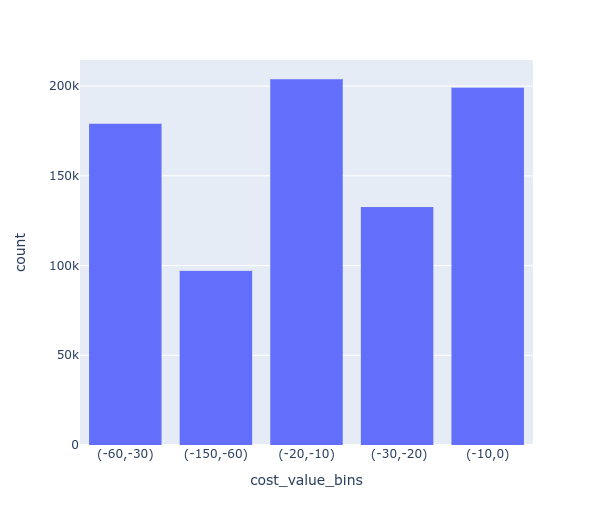
\includegraphics[width=\textwidth]{obrazky/grafy/histogram/newplot(2).png}
      \vspace*{-3em}
      \caption{Histogram pro hodnoty \\ velikosti shrinku v peněžních jednotkách.}
      \label{obr:nb:hist}
    \end{minipage}%
    \hspace*{-2em}
    \begin{minipage}[b]{.55\textwidth}
        \centering
        \captionsetup{justification=centering}
        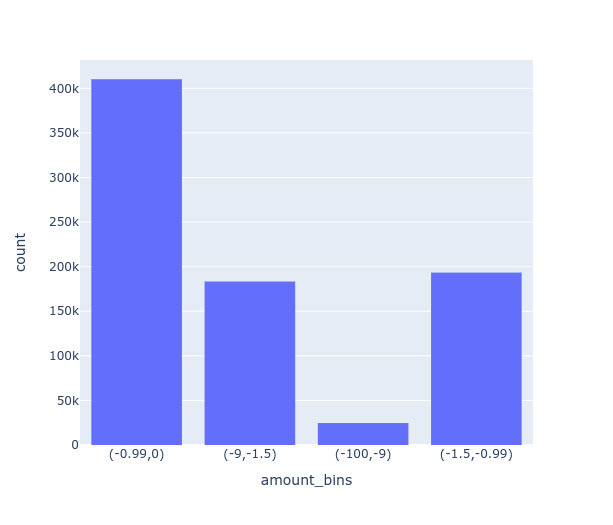
\includegraphics[width=\textwidth]{obrazky/grafy/histogram/newplot(1).png}
        \vspace*{-3em}
        \caption{Histogram pro hodnoty \\ objemu shrinku v kusech.}
        \label{obr:nb:hist2}
    \end{minipage}
    \vspace*{-2em}

\end{figure}


\begin{figure}[h!]
    \centering
    \begin{minipage}[b]{.55\textwidth}
      \centering
      \captionsetup{justification=centering}

      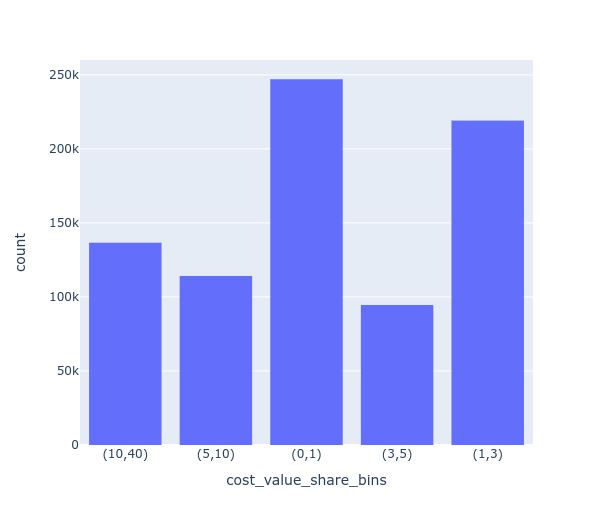
\includegraphics[width=\textwidth]{obrazky/grafy/histogram/newplot.png}
      \vspace*{-3em}
      \caption{Histogram podílu shrinku \\na tržbách shrinkovaného produktu.}
      \label{obr:nb:hist3}
    \end{minipage}%
    \hspace*{-2em}
    \begin{minipage}[b]{.55\textwidth}
        \centering
        \captionsetup{justification=centering}
  
        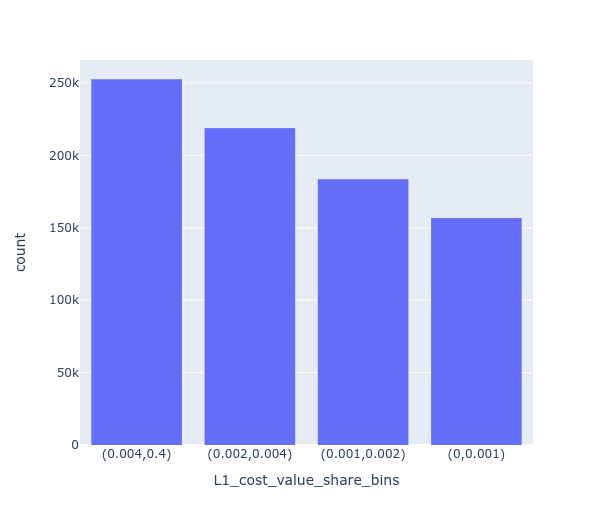
\includegraphics[width=\textwidth]{obrazky/grafy/histogram/newplot(3).png}
        \vspace*{-3em}
        \caption{Histogram podílu shrinku \\a tržeb v kategorii úrovně 1.}
        \label{obr:nb:hist4}
    \end{minipage}     
       \vspace*{-1em}
\end{figure}

\begin{figure}[h!]
        \centering
        \captionsetup{justification=centering}
        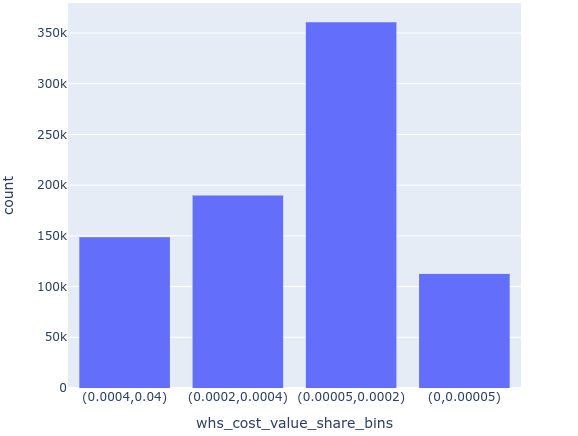
\includegraphics[width=0.55\textwidth]{obrazky/grafy/histogram/newplot(4).png}
        \caption{Histogram podílu shrinku \\na celkových tržbách prodejny.}
        \label{obr:nb:hist5}
        \vspace*{-1em}
\end{figure}

Pro první hypotézu je uvedeno volání funkce v jazyce Python včetně předaných parametrů. Rovněž je v tabulce uvedený celý výstup v obdobném formátu jako je zobrazen na konzoli po ukončení běhu funkce. Dále už kódy, ani přesné výstupy uvedené nebudou, ale bude uveden pouze popis vstupů a komentář k výstupům. 

\section{Hypotézy}

Před spuštěním metody bylo vždy třeba vznést hypotézu, která by mohla být pravdivá pro data týkající se shrinků. Tuto hypotézu pak přeformulovat do podoby asociačního pravidla, jehož pravdivost  na vstupních datech ověřuje metoda \emph{4ftMiner}. Tato metoda se předá jako parametr funkci \texttt{cleverminer}. Pravidlo se funkci zadává pomocí parametrů jako jednotlivé cedenty - antecedenty, sukcedenty, případně podmínky. Více o principu metody je ovedeno v teoretické části práce.

\vspace*{1em}

\textbf{Hypotéza č. 1: Objem prošlého zboží je závislý na typu promoakce a dni v týdnu}

Ve zkoumaných datech je zboží bez promoakce zastoupeno $58{,}2$ \%, zboží týden po evidované promoakci $23{,}2$ a zboží v promoakci $18{,}6$ procentem. 

Asociační pravidlo má tvar:
\begin{equation}
    \varphi_{\mbox{\,\footnotesize Den v týdnu}} \land \varphi_{\,\mbox{\footnotesize Typ promoakce}} \Rightarrow \psi_{\mbox{\,\footnotesize Množství}}
\end{equation}

V ukázce kódu \ref*{code:cleverminerH1} jsou uvedené parametry pro spuštění metody. Konfidence byla zvolena 80 \%. Výsledky běhu jsou uvedené v tabulce \ref*{tab:H1vysl}. Z této tabulky lze vyčíst, že pro vybrané dny v týdnu -- pondělí, úterý, středa, čtvrtek a neděle, tj. nikoli pro pátek a sobotu -- a pro produkty, které byly v den záznamu týden po promoakci platí, že 80 \% těchto záznamů bylo v množství do jednoho kusu. To znamená, že se jedná o produkty, které jsou vážené. Jejich přepočet na kusovou jendotku tedy může být menší než jeden celý kus. Podle dalšího zkoumání dat jsem zjistila, že se jedná především o kategorii \emph{Masné výrobky} ze třetí úrovně hierarchie.


\begin{lstlisting}[language=Python, style=mystyle, label={code:cleverminerH1}, caption={Hypotéza č. 1, funkce \texttt{cleverminer}.}]
cleverminer(df = data,
            proc = "4ftMiner", 
            quantifiers = {"conf":0.8, "Base":1000},
            ante = {
                    "attributes":
                    [
                        {
                            "name":"weekday", 
                            "type":"seq", 
                            "minlen":1, "maxlen":3
                        },
                        {
                            "name":"promo", 
                            "type":"sec", 
                            "minlen":1, "maxlen":1
                        }
                    ], 
                    "minlen":2, "maxlen":2, "type":"con"
                    },
            succ = {
                    "attributes":
                    [
                        {
                            "name":"amount_bins", 
                            "type":"subset", 
                            "minlen":1, "maxlen":1
                        }
                    ], 
                    "minlen":1, "maxlen":1, "type":"con"
                    }
            )
    \end{lstlisting}

    \begin{table}[h!]
        \begin{center}
                \captionsetup{justification=centering}
        \caption{Výstup funkce \texttt{cleverminer} pro hypotézu 1.}
        \begin{tabular}{rrrp{7.5cm}}
            Základ ($a$) & Konfidence & AAD & AP [\%]\\
            \midrule
19765 & 0.821 & $+0.623$ & weekday(0) $\land$  promo(after\_promo) $\Rightarrow$ amount\_bins((-0.99,0)) \\
39271 & 0.820 & +0.622 & weekday(0, 1)  $\land$ promo(after\_promo) $\Rightarrow$ amount\_bins((-0.99,0)) \\
63920 & 0.815 & +0.613 & weekday(0, 1, 2)  $\land$ promo(after\_promo) $\Rightarrow$ amount\_bins((-0.99,0)) \\
19506 & 0.820 & +0.621 & weekday(1)  $\land$ promo(after\_promo) $\Rightarrow$ amount\_bins((-0.99,0)) \\
44155 & 0.813 & +0.608 & weekday(1, 2)  $\land$ promo(after\_promo) $\Rightarrow$ amount\_bins((-0.99,0)) \\
68666 & 0.810 & +0.603 & weekday(1, 2, 3)  $\land$ promo(after\_promo) $\Rightarrow$ amount\_bins((-0.99,0)) \\
24649 & 0.808 & +0.598 & weekday(2)  $\land$ promo(after\_promo) $\Rightarrow$ amount\_bins((-0.99,0)) \\
49160 & 0.806 & +0.595 & weekday(2, 3)  $\land$ promo(after\_promo) $\Rightarrow$ amount\_bins((-0.99,0)) \\
24511 & 0.805 & +0.593 &weekday(3) $\land$ promo(after\_promo) $\Rightarrow$ amount\_bins((-0.99,0)) \\
18864 & 0.813 & +0.608 &weekday(6)  $\land$ promo(after\_promo) $\Rightarrow$ amount\_bins((-0.99,0)) \\
       
            \end{tabular}
        \label{tab:H1vysl}
    \end{center}
    \end{table}

\subsubsection*{Hypotéza č. 2: Kategorie shrinkovaného zboži je závislá na typu promoakce a dni v týdnu}

Asociační pravidlo má tvar:
\begin{equation}
    \varphi_{\mbox{\,\footnotesize Den v týdnu}} \land \varphi_{\,\mbox{\,\footnotesize Typ promoakce}} \Rightarrow \psi_{\mbox{\,\footnotesize Hierarchie3}} \lor \psi_{\mbox{\,\footnotesize Hierarchie4}},
\end{equation}
kde označením Hierarchie3 jsou myšleny kategorie na třetí úrovni produktové hierarchie, obdobně pro pojem Hierarchie4.

Parametry předané funkci jsou podobné jako u předchozí hypotézy.

\subsubsection*{Hypotéza č. 3: Na některých lokalitách vyhazují často stejné produkty}

Asociační pravidlo má tvar:
\begin{equation}
    \varphi_{\mbox{\,\footnotesize Typ prodejny}} \land \varphi_{\,\mbox{\footnotesize Okres}} \Rightarrow \psi_{\mbox{\,\footnotesize Množství}}
\end{equation}

(úroveň hierarchie 3). 
60 \% záznamů týkajících se okresů Jindřichův Hradec, Ústí nad Labem, Písek nebo Strakonice tvoří shrinky z kategorie \emph{Masné výrobky}. Pro záznamy z okresu Kladno, které jsou zároveň evidovány velkými prodejnami kategorie Masné výrobky byla zastoupena až téměř 70 \%. Necelými 70 \% je tato kategorie zastoupená také v záznamech v malých prodejnách v okrese Praha-východ.

Pokud úplně vynecháme kategorie Masné produkty ze vstupních dat, pak se nejčastěji ve výsledcích objevovala kategorie \emph{Pečivo}. Pro záznamy z velkých prodejen v okrese Pardubice nebo Plzeň-město Pečivo zaujímalo přes 60 \% těchto záznamů. Nad 50 \% záznamů pro okresy Bruntál, Olomouuc, Příbram nebo Uherské Hradiště. 50 \% záznamů náleželo kategroii Pečivo také v záznamech z malých prodejen v okrese Klatovy, Náchod nebo Přerov.

Po vynchání kategorie Pečivo již dostáváme maximální konfidenci 33 \%, a to pro kategorii Zelenina ve zbylých záznamech z okresu Ostrava-město, Kroměříž, Hradec Králové nebo Karvinná.


\subsubsection*{Hypotéza č. 3: Na některých v některých lokalitách mají často zaznamenaný shrink}

Tvar asociačního pravidla:
\begin{equation}
    \varphi_{\mbox{\,\footnotesize Okres}} \land \Rightarrow \psi_{\mbox{\,\footnotesize Podíl na prodejně}}
\end{equation}



\subsubsection*{Hypotéza č. 4: Některé produkty se vyhazují častěji než jiné, ale v malém množství.}

 Kategorie MEAT PRODUCTS (PROC. MEAT SERVICE)-( masné produkty, šunka, salámy, klobásy) byla zaznamenána téměř 300 tisíckrát, a v 90 procentech se jednalo o množství odpovídající do jednoho balení. 
%   Jedná o vážené pultové produkty - jde o
 Pokud se vyhazují čerstvé ryby (fresh fish), tak v 94 
\% záznamů je to množství do jednoho kusů. Tapas se vyhazují v 89 \% po jednom kusu (obvykle se jedná o sendviče a bagety)
Kategorie vejce se vyhazuje v 82 \% po jednom kusu balení
Kategorie pečiva se vyhazuje v 56 \% v počtu kusů do 10 ks v až 94 tis. záznamech.
Kategorie CORE FRUIT (hrušky a jablka) se vyhazuje 74 \% případech záznamů (14 000 záznamů) v množství do jednoho kusu - váhový přepočet.

\subsubsection*{Hypotéza č. 5: Některé vyhazované kategorie produktů jsou výrazně nákladnější.}

Pokud se vyhazují čerstvé ryby (fresh fish), tak v téměř 80 \% případech záznamů jsou ztracené náklady vyšší  - 60-150 balení.
Pokud se vyhazuje kategorie Red meat, tak z téměř 60 \% ve větším množství - 60-150 balení.
Kategorie CHILLED PRODUCT SERVICE, která obsahuje čerstvé chlebíčky, saláty a pochutiny na pultovém prodeji, se v 50 \% vyhazují v množství

\subsubsection*{Hypotéza č. 6: Shrink některých produktů je v porovnání s tržbami těchto produktů na stejné prodejně velký.}

Nejedná se o porovnání s celkovými tržbami prodejny, ale pouze o týdenní tržbu těch produktů, které měli zaznamenaný v daném týdnu shrink.
Tapas se mají share shrinku v 84 \% zaznamenaných případech mezi 10-40 \%.
 Cukrářské výrobky  mají share shrinku v 74 \% zaznamenaných případech mezi 10-40 \%.
 Banány mají share shrinku v 80 \% zaznamenaných případech do 1 \%.
 Více než 30 tis. záznamů je u Citrusů, Jablek a hrušek a v okolo 65 \% je share shrinku do 1 \%.

 Pokud mezi produkty, kterým byl zaznamenán dražší (30-60 Kč) shrink, jsou jogurty, tak jejich share shrinku na tržbách je mezi 10-40 \%, totéž se týká Tapas.
Pokud mezi produkty, kterým byl zaznamenán levný (do 10 Kč) shrink, je ovoce, tak jejich share shrinku na tržbách je do 1 \%, totéž se týká in kořenové zeleniny.

\subsubsection*{Hypotéza č. 7: Kategorie má vliv na zastoupení shrinku na celkových tržbách prodejny v dané kategorii úrovně 1.}

S pracděpodobností vyšší než 50 \% se toto tvrzení potvrdilo pouze u kategorie Bylinky z úrovně 4. Kdy (0.002,0.005).

\subsubsection*{Hypotéza č. 8: Den v týdnu nebo čtvrtina měsíce mají vliv na záznamy.}

Ve středu, čtvrtek a pátek v poslední čtvrtině měsíce je dvakrát více záznamů než v jiných dnech. Ostatní části měsíce jsou konzistentní.